% !TeX spellcheck = da_DK
\subsection{Software}
Patienternes data skal behandles i form af grafisk visualisering, jævnfør afsnit \ref{subsec:software} på side \pageref{subsec:software}. Derudover skal patienternes resultater i forbindelse med testen kunne gemmes til analyse og senere brug. Dette sker ved, at det analoge signal konverteres til et digitalt signal og indsendes igennem USB-isolatoren til en computer. For at imødekomme disse krav anvendes en computer med programmet Matlab. I Matlab designes en GUI (Graphical User Interface), hvor signalet fra accelerometeret visualiseres. Signalet optages i Matlab via NIDAQ'en. Grunden til, at der designes en GUI, er for at optimere brugervenligheden. I GUI'en ses en graf, samt fire knapper og en toolbar, dette er illustretet på \figref{Fig:GUI_generisk}. 
\begin{figure}[H] 
	\centering 
	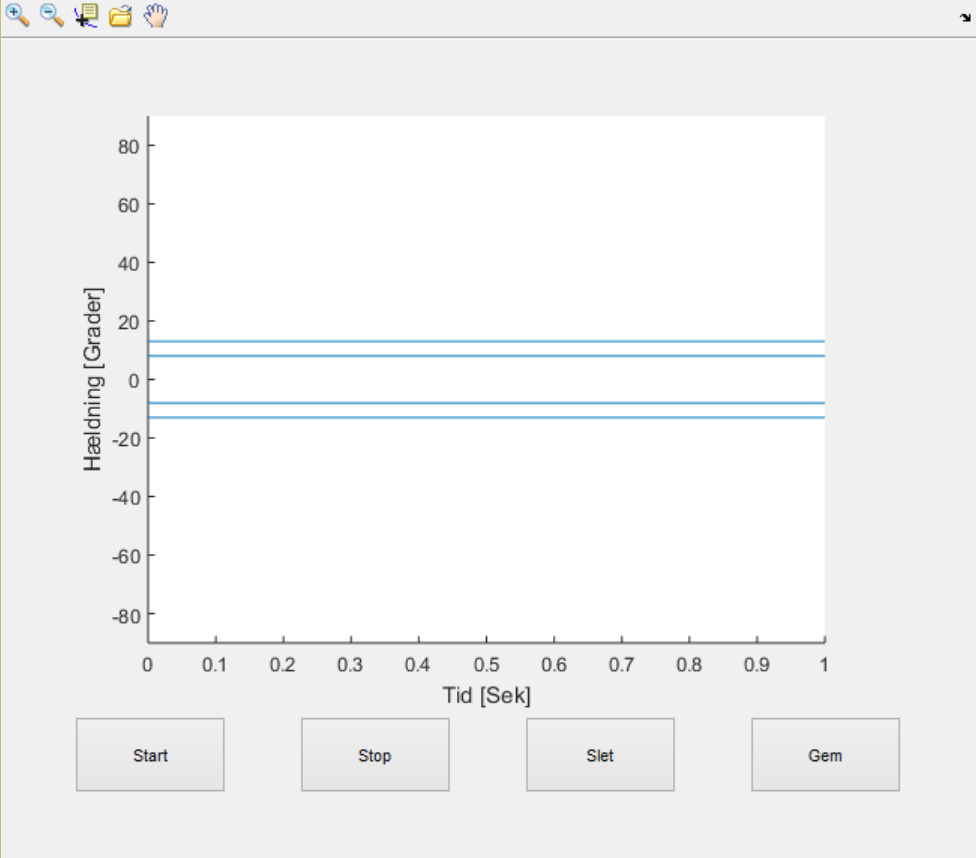
\includegraphics[scale=0.5]{figures/cProblemloesning/GUI_generisk.PNG}
	\caption{Af figuren fremgår GUI'ens display.De blå linjer illustrer de forskellige tærkselværdier i positiv og negativ retning for hhv. $\pm 8\circ$ og $\pm 13\circ$.}
	\label{Fig:GUI_generisk}
\end{figure} 
I koordinatsystemet måler y-aksen hældningen i grader, mens x-aksen måler tiden i sekunder. Dette gør det enkelt at se hvilken side patienten hælder til, samt i hvor lang tid patienten har befundet sig i denne position.
De fire blå linjer på tværs af koordinatsystemet er de opstillede tærskelværdier for den gule og røde LED, som skal lyse i hhv. $\pm 8\circ$ og $\pm 13\circ$. Derved synliggøres de grænser der er for patienten, hvorved personalet herudfra kan vurdere patientens balance. I displayet er der en start-, stop-, slette- og gemmefunktion.
I toolbaren er der flere knapper, disse har til opgave at gøre det muligt at manipulere med grafen. Forstørrelsesglaset med plusset gør det muligt at zoome ind på grafen, mens forstørrelsesglaset med minusset gør det muligt at zoome ud igen. Knappen med et papir og et plus gør det muligt at aflæse det præcise punkt på grafen der markeres. Den åbne mappe gør det muligt at åbne en fil i GUI'en og hånden gør det muligt at panorere i grafen.
For at benytte GUI'en skal det fagkyndige personale følge fremgangsmåden på \ref{Fig:fremgangsmåde_software}.
\begin{figure}[H] 
	\centering 
	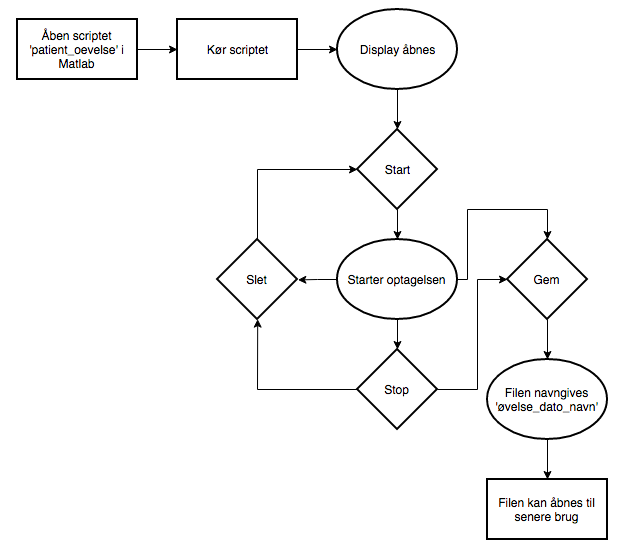
\includegraphics[scale=0.5]{figures/cProblemloesning/Software_flowdiagram.PNG}
	\caption{Flowdiagrammet viser fremgangsmåden for personalet til at benytte softwaren}
	\label{Fig:fremgangsmåde_software}
\end{figure}


Krav:
ˆ Skal kunne fremvise data med information om patientens hældning i de enkelte øvelser,
herunder hvor ofte patienten har bevæget sig ud i risikozonerne.
ˆ Skal kunne gemme data med information om patientens hældning.
Tolerance:
ˆ Der accepteres ingen afvigelse ift. software.

\subsubsection{Test}
Softwaren testes ved en måling på XX sekunder. Målingen sker ved at holde accelerometer i XX sekunder ved de forskellige tærskelværdier. For at optage signalet følges fremgangsmåden på \ref{Fig:fremgangsmåde_software}. Efter optagelsen gemmes signalet.

%Her skal det testes, hvorvidt systemet kan hvad vi beskriver det skal kunne.
%- Opsamling af noget data, hvor vi efterfølgende tester om programmet behandler dataen som det var tænkt.



%Vi kunne for at gøre programmet mere brugervenligt udarbejde en manual til systemet. Derudover kunne det være fordelagtigt at det fagkyndige personalet at have mulighed for at ændre akserne, og her tænkes specielt tidsaksen. Dette tænkes da systemet skal kunne optage selvtræning og da det ikke forventes at patienten tænder og slukker systemet efter hver enkelt øvelse. Dette vil både være svært at huske for patientgruppe (gamle og måske med kognitive komplikationer) og så ville de måske glemme at slå den til igen. Derfor tænkes det at de lader systemet optage signaler under hele selvtrænings sessionen. Det vil midlertidigt blive til utrolig meget data, hvor en stor del af dataen vil være pauser for patienten og derved ubrugelig data for det fagkyndige personale. Det ville derfor være smart at hvis de forholdsvis nemt kunne udvælge perioder i dataen, de gerne vil undersøge nærmere. 
%Derudover skal vi også have gjort patienten og det fagkyndige personale opmærksomme på hvilken øvelse der foretages!
%Det kunne måske være en ide, at vi i grafen kunne ligge tærskelværdierne ind som en form for linjer, så det blev nemmere at aflæse grafen
%Skal vi have en løbende visning af signalet i en graf eller er det bare til sidst! 

%Vores program skal altså kunne:
%  -Optage signalet
% - Behandle signalet således, alt efter sværhedsgrad 
%  - Plotte signalet
% - Gem data'en 
